\begin{defi}{Partie dense}
    \marginnote[0cm]{Source : \href{https://www.bibmath.net/dico/index.php?action=affiche&quoi=./d/dense.html}{Partie dense -- \textsf{Bibm@ath.net}}}
    Soit $E$ un espace vectoriel normé et $D$ une partie de $E$. On dit que $D$ est \emph{dense} dans $E$ si l'une des conditions équivalentes suivantes est vérifiée:
    \begin{itemize}
        \item pour tout $x \in E$, il existe une suite $(y_n)$ d'éléments de $D$ qui converge vers $x$,
        \item pour tout $x \in E$, pour tout $\varepsilon > 0$, il existe $y \in D$ tel que $\norme{y - x} \leqslant \varepsilon$,
        \item l'adhérence $\overline{D}$ de $D$ est égale à $E$.
    \end{itemize}
\end{defi}

\subsection{Le cas des matrices inversibles}

\begin{theo}{Densité de $\Gl_n(\C)$ dans $\M_n(\C)$}
    L'ensemble des matrices inversibles de $\M_n(\C)$ est dense dans $\M_n(\C)$.
\end{theo}

\begin{preuve}
    Soit $A \in \M_n(\C)$. Son polynôme caractéristique $\chi_A$ est de degré $n$ et admet donc au plus $n$ racines. \\
    Notons $r \defeq \min \big\{ |\lambda|, \lambda \in \Sp(A) \setminus \{0\} \big\}$. \\
    Ainsi,
    $$\forall t \in ]0,r[,\ \chi_A(t) \not= 0$$ 
    soit 
    $$\forall t \in ]0,r[,\ A - t \I_n\in \Gl_n(\C).$$
    Soit $p_0 \defeq \min \left\{ p\ \middle|\ \frac{1}{p} < r \right\}$. Ainsi, en posant
    $$A_p \defeq A - \frac{1}{p + p_0} \I_n,$$
    la suite $(A_p)_{p \geqslant 0}$ est une suite de matrices inversibles qui converge vers la matrice $A$. \\
    Finalement, pour toute matrice $A \in \M_n(\C)$ nous avons construit une suite de matrices inversibles qui converge vers la matrice $A$, ce qui assure la densité de $\Gl_n(\C)$ dans $\M_n(\C)$.
\end{preuve}

\begin{marginfigure}[-8cm]
    \centering
    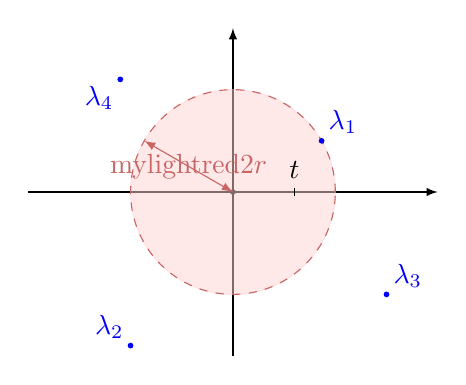
\begin{tikzpicture}[scale=1.3]
  \definecolor{mylightred}{RGB}{255,210,210}
  \definecolor{myred}{RGB}{200,100,100}
  \definecolor{mylightred2}{RGB}{255,232,232}
      \def\ang{150}
      \def\R{1}
      \coordinate (O)  at (0, 0);
      \coordinate (L1) at (30:1);
      \coordinate (L2) at (-1, -1.5);
      \coordinate (L3) at (1.5, -1);
      \coordinate (L4) at (1.2, 1);
      \coordinate (L5) at (-1.1, 1.1);
     
      \draw[-latex] (0, -1.6) -- (0, 1.6);
      \draw[-latex] (-2, 0) -- (2, 0);
      \fill[radius=0.8pt,black] (O) circle;
      \draw[mylightred, fill, opacity=0.5] (O) circle (\R);
      \draw[myred, dashed] (O) circle (\R);
      \fill[radius=0.8pt,blue]
        (L1) circle node[above right=-1pt] {$\lambda_1$}
        (L2) circle node[above left =-1pt] {$\lambda_2$}
        (L3) circle node[above right=-1pt] {$\lambda_3$}
        (L5) circle node[below left =-1pt] {$\lambda_4$};
      \draw (0.6, -0.04) -- (0.6, 0.04)  node[above] {$t$};
      \draw[latex-latex, myred] (O) -- (\ang:\R) node[midway] {\contour{mylightred2}{$r$}};
\end{tikzpicture}
\end{marginfigure}

\begin{exercice}
    Soit $A, B \in \M_n(\K)$. Montrer que $\chi_{AB}=\chi_{BA}$. \\
    On pourra commencer par le cas où la matrice $A$ est inversible.
\end{exercice}

La démonstration suivante est \say{ chimique }: la continuité du déterminant va servir de catalyseur à la partie dense qu'est $\Gl_n(\K)$ dans $\M_n(\K)$.
\marginnote[0cm]{Une application continue est entièrement déterminée par l'image d'une partie dense}

\begin{solution}
    \begin{itemize}
    \item[$\rhd$] On suppose que la matrice $A$ est inversible. Revenons à l'expression du polynôme caractéristique par le déterminant:
        \begin{align*}
        \chi_{AB} &= \det(\lambda \I_n - AB) \\
        &= \det(A(\lambda \Inv{A} - B)) &\text{car } A \in \Gl_n(\K) \\
        &= \det(A) \det(\lambda \Inv{A} - B) &\text{ par multiplicité du déterminant} \\
        &= \det(\lambda \Inv{A} - B) \det(A) \\
        &= \det(\lambda \I_n - BA) \\
        \chi_{AB} &= \chi_{BA}
    \end{align*}
    \item[$\rhd$] Revenons au cas général. Soit $A \in \M_n(\K)$. D'après la densité des matrices inversibles dans $\M_n(\K)$, il existe une suite $(A_p)_{p \in \N}$ de matrices inversibles qui converge vers la matrice $A$. D'après le premier point, pour tout $p \in \N$,
    $$\chi_{A_p B} = \chi_{B A_p}$$
    soit 
    $$\det(\lambda \I_n - A_p B) = \det(\lambda \I_n - B A_p).$$
    Comme le produit matriciel est une application bilinéaire, la matrice $A_p B$ (resp. $B A_p$) tend vers $AB$ (resp. $BA$) quand $p$ tend vers l'infini. \\ De plus, comme le déterminant est une application multilinéaire en dimension finie, elle est continue et 
    $$\det(\lambda \I_n - A B) = \det(\lambda \I_n - B A)$$
    soit 
    $$\chi_{A B} = \chi_{B A}.$$
    \end{itemize}
\end{solution}

Ce résultat peut être montré par un argument plus \say{ mécanique }. \\
Soient $A, B \in \M_n(\K)$. Pour tout $\lambda \in \K$, on pose
$$
U \defeq
\begin{pmatrix}
    A & \lambda \I_n \\
    \I_n & B
\end{pmatrix}
\text{ et }
V \defeq 
\begin{pmatrix}
    B & -\lambda \I_n \\
    -\I_n & 0_n
\end{pmatrix}.
$$
On calcule alors
$$UV = 
\begin{pmatrix}
    AB - \lambda \I_n & \bigstar \\
    0 & -\lambda \I_n
\end{pmatrix}
\quad
VU = 
\begin{pmatrix}
    BA - \lambda \I_n & 0 \\
    \bigstar & -\lambda \I_n
\end{pmatrix}.
$$
Comme $\det(UV) = \det(VU)$, on obtient
$$(-\lambda)^n \det(AB - \lambda \I_n) = (-\lambda)^n \det(BA - \lambda \I_n).$$
En particulier on obtient:
$$\forall \lambda \not= 0,\ \det(AB - \lambda \I_n) = \det(BA - \lambda \I_n)$$
et l'égalité est triviale si $\lambda = 0$. \\
On a donc montré que 
$$\chi_{A B} = \chi_{B A}.$$

\begin{prop}{}
    $\Gl_n(\R)$ est un ouvert de $\M_n(\R)$.
\end{prop}

\begin{preuve}
    
\end{preuve}

\begin{prop}{}
    $\M_n(\R) \setminus \Gl_n(\R)$ est fermé mais non compact (pour $n \geqslant 2$).
\end{prop}

\subsection{Le cas des matrices diagonalisables}

\begin{theo}{Densité de l'ensemble des matrices diagonalisables dans  $\M_n(\C)$}
    L'ensemble des matrices diagonalisables de $\M_n(\C)$ est dense dans $\M_n(\C)$.
\end{theo}

\begin{preuve}
    Soit $M \in \M_n(\C)$. Cette matrice est trigonalisable puisque son polynôme caractéristique est scindé sur $\C$ d'après le théorème de \textsc{d'Alembert}-\textsc{Gauss}. On note $\lambda_1, \dots, \lambda_s$ ses valeurs propres distinctes et $r_1, \dots, r_s$ les multiplicités associées. Il existe donc une matrice $P \in \Gl_n(\C)$ telle que
    $$
    M = P
    \begin{pmatrix}
        \lambda_1 & & & t_{i,j} \\
        0 & \ddots & & \\
        \vdots & \ddots & \ddots & \\
        0 & \cdots & 0 & \lambda_s
    \end{pmatrix}
    \Inv{P} \defeq P T \Inv{P}.
    $$
    Soit $\varepsilon > 0$, nous allons commencer par \say{ séparer } les valeurs propres distinctes. On peut trouver un rayon $\rho$ tel que $0 < \rho < \varepsilon$, pour lequel les disques $D(\lambda_1, \rho), \dots, D(\lambda_s, \rho)$ sont distincts deux à deux. Enfin, dans chacun de ces disques -- qui sont des parties infinies de $\C$ -- on peut, pour tout $i \in \llbracket 1, s \rrbracket$, choisir $r_i$ complexes notés $\lambda_{i,1}, \dots, \lambda_{i,r_i}$ distincts deux à deux. \\
    On peut même expliciter
    $$\lambda_{i,1} \defeq \lambda_i + \frac{\rho}{1}, \dots, \lambda_{i, r_i} \defeq \lambda_i + \frac{\rho}{r_i}.$$ 
    
    \begin{figure*}[h!]
        \centering
        \begin{tikzpicture}[scale=0.8]
  \definecolor{mylightred}{RGB}{255,210,210}
  \definecolor{myred}{RGB}{255,0,0}
  \definecolor{mydarkred}{RGB}{140,40,40}

  \begin{scope}[local bounding box=struct, scale=2]
      \def\ang{15}
      \def\R{0.35}
      \coordinate (O)  at (0, 0);
      \coordinate (L1) at (0.4, 0.38);
      \coordinate (L2) at (2, 0.5);
      \coordinate (L3) at (0.5, -0.5);
      \coordinate (L4) at (1, 1);
      \coordinate (L5) at (-0.5, 0.5);
     
      \draw[-latex] (0, -1) -- (0, 1.5);
      \draw[-latex] (-1, 0) -- (2.5, 0);
      \fill[radius=0.5pt,black] (O) circle;
      \foreach \i in {1, ..., 5}{
         \draw[mylightred, fill] (L\i) circle (\R);
         \draw[myred] (L\i) circle (\R);
      }
      \fill[radius=0.8pt,blue]
        (L1) circle node[above left=-2pt] {$\lambda_1$}
        (L2) circle node[above left=-2pt] {$\lambda_2$}
        (L3) circle node[above left=-2pt] {$\lambda_3$}
        (L4) circle node[above left=-2pt] {$\lambda_4$}
        (L5) circle node[above left=-2pt] {$\lambda_5$};
  \end{scope}
  
  \def\RL{2}
  \begin{scope}[shift={($(struct.east)+(2.5,0)$)}, scale=1]
      \coordinate (L2) at (-3.5, 0.5);
      \def\R{0.7}
      \def\angrho{15}
      \coordinate (O)  at (0,0);
      \coordinate (R) at (\angrho:\RL);
      \foreach \k in {1, ..., 5}{
          \coordinate (Z\k) at (360/5*\k-30:\RL/\k);
      }
      \draw[mylightred, fill] (O) circle (\RL);
      \draw[myred] (O) circle (\RL) node[above=45pt] {$D(\lambda_2, \rho)$};
      \fill[radius=0.8pt,mydarkred]
        (Z1) circle node[above right=-1pt,scale=0.75] {$\lambda_{2, 1}$}
        (Z2) circle node[above           ,scale=0.75] {$\lambda_{2, 2}$}
        (Z3) circle node[above left=-1pt ,scale=0.75] {$\lambda_{2, 3}$}
        (Z4) circle node[below           ,scale=0.75] {$\lambda_{2, 4}$}
        (Z5) circle node[below right=-1pt,scale=0.75] {$\lambda_{2, 5}$};
      \foreach \i in {1, ..., 5}{
        \draw[black, dotted] (O) -- (Z\i);
      }
      \fill[radius=2.0pt,blue] (O) circle node[above left=1pt] {\contour{mylightred}{$\lambda_2$}};
      \draw[latex-latex, mydarkred] (O) -- (R) node[midway] {\contour{mylightred}{$\rho$}};
      
      \tkzDefExtSimilitudeCenter[R](O,\RL)(L2,\R) \tkzGetPoint{J}
      \tkzDefTangent[from  with R= J](O,\RL) \tkzGetPoints{F}{G}
      \tkzDefTangent[from with R= J](L2,\R)  \tkzGetPoints{F'}{G'}
      \tkzDrawSegments[dashed, color=myred, thin, arrowMe=latex'](F',F G',G)
  \end{scope}
  
\end{tikzpicture}
        \caption*{\centering Représentation des disques $D(\lambda_i, \rho)$ et des complexes choisis à l'intérieur. Les $\lambda_{2, i}$ sont décalés pour une meilleure lisibilité.}
    \end{figure*}
    
    On considère alors la matrice
    $$M_\varepsilon \defeq P 
    \begin{pmatrix}
        \lambda_{1, 1} & & & t_{i,j} \\
        0 & \ddots & & \\
        \vdots & \ddots & \ddots & \\
        0 & \cdots & 0 & \lambda_{s, r_s}
    \end{pmatrix}
    \Inv{P} \defeq P T_\varepsilon \Inv{P}.
    $$
    Par construction, cette matrice de $\M_n(\C)$ possède $n$ valeurs propres distinctes, elle est donc diagonalisable. \\
    On choisit maintenant sur $\M_n(\C)$ la \emph{norme du $\sup$} sur les coefficients, définie par:
    $$\forall M \defeq (m_{i,j})_{1 \leqslant i, j \leqslant n} \in \M_n(\C),\ \norme{M} = \max_{1 \leqslant i, j \leqslant n} |m_{i,j}|.$$
    On démontre facilement que pour $A, B \in \M_n(\C)$, $\norme{AB} \leqslant n \norme{A} \norme{B}$ \note. Ainsi
    \marginnote[0cm]{
        \note pour tout $(i, j) \in \llbracket 1, n \rrbracket^2$,
        \begin{align*}
            \big| [AB]_{i,j} \big| &= \left|\sum_{k=1}^n a_{i,k} b_{k,j} \right| \\
            &\leqslant \sum_{k=1}^n |a_{i,k}| |b_{k,j}| \\
            &\leqslant \sum_{k=1}^n \norme{A} \norme{B} \\
            &\leqslant n \norme{A} \norme{B}.
        \end{align*}
        Cette norme est presque sous-multiplicative.
    }
    $$\norme{M - M_\varepsilon} = \norme{P (T - T_\varepsilon) \Inv{P}} \leqslant \underbrace{n \norme{P} \norme{P^{-1}}}_{\defeq K} \norme{T - T_\varepsilon} \leqslant K \varepsilon.$$
    En effet, 
    $$
    T - T_\varepsilon = 
    \begin{pmatrix}
    \lambda_1 - \lambda_{1, 1} &  & \\
    & \ddots & \\
    & & \lambda_s - \lambda_{s, r_s}
    \end{pmatrix}
    $$  
    donc
    $$\norme{T - T_\varepsilon} = \max_{1 \leqslant i \leqslant n} |\lambda_i - \lambda_{i, r_i}|.$$
    Or les $\lambda_{i, r_i}$ ont été choisis dans les disques $D(\lambda_i, \rho)$ et donc pour tout $i \in \llbracket 1, n \rrbracket$,
    $$\big|\lambda_i - \lambda_{i, r_i}\big| \leqslant \rho < \varepsilon.$$
    Ceci achève la démonstration, puisque si $\varepsilon$ tend vers $0$, la matrice $M_\varepsilon$ tend vers la matrice $M$ pour la norme $\norme{\cdot}$ donc pour toute norme puisqu'en dimension finie, toutes les normes sont équivalentes.
\end{preuve}

\begin{exercice}
    Peut-on dire que l'ensemble des matrices diagonalisables dans $\M_n(\C)$ est dense dans $\M_n(\R)$ ?
\end{exercice}

\begin{prop}{}
    L'ensemble des matrices diagonalisables de $\M_n(\R)$ est connexe par arcs.
\end{prop}

\subsection{Divers}

\begin{exercice}
    Montrer que $\Ortho_n(\R)$ est compact. $\Ortho_n(\R)$ est-il convexe ?
\end{exercice}

\begin{solution}
    
\end{solution}

\begin{exercice}
    Montrer que $\Sym_n(\R)$ est fermé.
\end{exercice}

\begin{exercice}
    Soit $p \in \llbracket 0, n-1 \rrbracket$. Montrer que l'ensemble des matrices de rang inférieur ou égal à $p$ est un fermé de $\M_n(\R)$.
\end{exercice}

\begin{exercice}
    Montrer que l'ensemble des matrices stochastiques est un compact convexe de $\M_n(\R)$.
\end{exercice}